\documentclass[a4paper, 12pt]{article}
\usepackage[margin=0.8in]{geometry}
\usepackage{tikz}
\usepackage{scrextend}
\usetikzlibrary{automata,positioning}
\usepackage{graphicx}
\usepackage{pgfplots}


\title{Scotland Yard}
\author{Julian Loscombe and Ben Milne}

\begin{document}
\maketitle
\section{Game Tree}
We have set up our game tree to use Alpha - Beta pruning in order to increase the depth that we can search to in the allotted time. In doing so we reduced the time to get to depth 4 from ???ms to ??? ms. In addition we are removing the double and secret moves from the game tree to further reduce the time to move through the trees. This is important because below a depth 6 search we would not even be considering some detectives moves when deciding what to do. A higher search depth also allows us to make mores with much greater foresight, something that is the hallmark of a competent player.
\subsection{Scoring}
To score our game state we use to main sources of information, the PageRank of the detectives' locations vs Mr X's location and the average (minimum?) distance between the detectives and Mr X using Dijkstras. We weight the PageRanks influence depending on Dijkstras because if the detectives are close, it is much more important to widen that distance than to get to an opportunistic node. In theory simply using Dijkstra would be sufficient as it itself uses PageRank, however, as the depth to which we can search is limited, using PageRank directly gives us some indication of advantageous positions.\\
\\
\begin{figure}[!h]
\centering
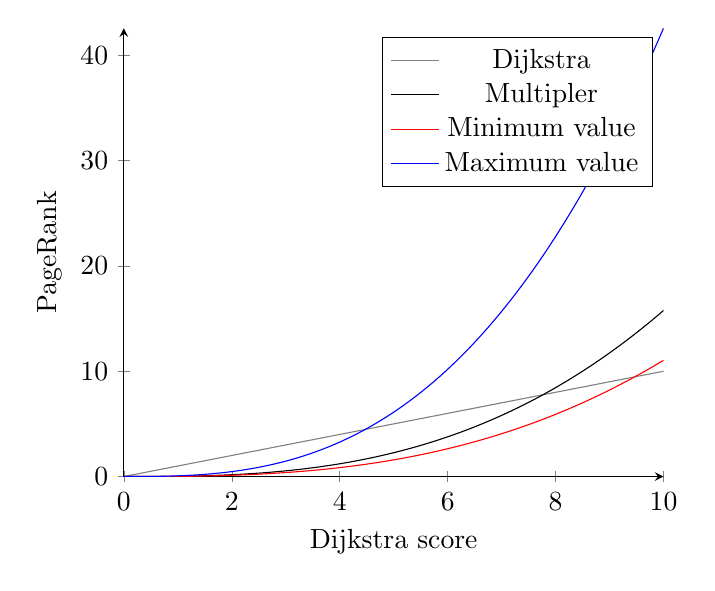
\begin{tikzpicture}
\begin{axis}[
    axis lines = left,
    xlabel = {Dijkstra score},
    ylabel = {PageRank},
]
%Below the red parabola is defined
\addplot [
    domain=0:10, 
    samples=100, 
    color=gray,
]
{x};
\addlegendentry{Dijkstra}
%Below the red parabola is defined
\addplot [
    domain=0:10, 
    samples=100, 
    color=black,
]
{(x^2.8)/40};
\addlegendentry{Multipler}
%Below the red parabola is defined
\addplot [
    domain=0:10, 
    samples=100, 
    color=red,
]
{((x^2.8)/40)*0.7};
\addlegendentry{Minimum value}
%Here the blue parabloa is defined
\addplot [
    domain=0:10, 
    samples=100, 
    color=blue,
    ]
    {((x^2.8)/40)*2.7};
\addlegendentry{Maximum value}
 
\end{axis}
\end{tikzpicture}
\end{figure}
\subsection{Threads}
Because we have multiple threads acting on our game tree at the same time we have had a sm�rg�sbord of difficult to trace errors. To fix this we have
\subsection{Iterative Depth Search}
Because we have a strict time limit in order to make our move and the initial conditions change the complexity of the game tree, we have decided to use an iterative depth search, updating the best move on each iteration and simply grabbing the one that is available when the time limit is approaching.
\subsection{Pruning}
We are hoping to keep the tree running throughout the game in order to use the work we have already done to extend the depth we are able to reach. Clearly though, we must prune branches that are made impossible by the game advancing in order to make any real progress. We achieve this by setting the root of the tree to be the node containing the last played move, thus making unneeded nodes unreachable. However, what if we are currently in one of those pruned branches? We would waste time evaluating nodes that are unnecessary. So, to avoid this,  we quickly traverse up the list when we enter our alphabeta() function to see if we are connected to the root node, if we are not we can simply return 0 immediately as it will make no difference to our final score.
\begin{figure}[h!]
  \centering
  	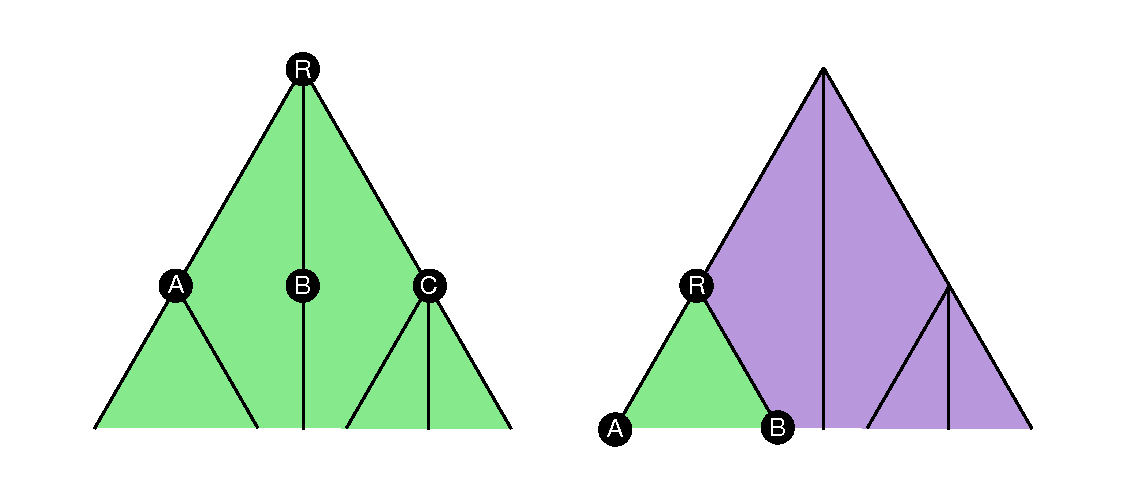
\includegraphics[width = 17cm]{TreePruning}\\
  \caption{After making move A, we can prune all other moves and their subsequent moves.}
\end{figure}
\end{document}